\renewcommand{\leveltopI}{-15cm + \leveltop}
\renewcommand{\leveltopII}{-15cm + \leveltopI}
\renewcommand{\leveltopIII}{-15cm + \leveltopII}
\renewcommand{\leveltopIIII}{-15cm + \leveltopIII}
\renewcommand{\leveltopIIIII}{-15cm + \leveltopIIII}
\renewcommand{\leveltopIIIIII}{-15cm + \leveltopIIIII}
\renewcommand{\leveltopIIIIIII}{-15cm + \leveltopIIIIII}
\renewcommand{\leveltopIIIIIIII}{-15cm + \leveltopIIIIIII}
\renewcommand{\leveltopIIIIIIIII}{-15cm + \leveltopIIIIIIII}
\renewcommand{\leveltopIIIIIIIIII}{-15cm + \leveltopIIIIIIIII}
\renewcommand{\leveltopIIIIIIIIIII}{-15cm + \leveltopIIIIIIIIII}
\renewcommand{\leveltopIIIIIIIIIIII}{-15cm + \leveltopIIIIIIIIIII}
\renewcommand{\leveltopIIIIIIIIIIIII}{-15cm + \leveltopIIIIIIIIIIII}
\begin{tikzpicture}[scale=.2, anchor=south]
\begin{scope}[yshift=\leveltopI cm]
\matrix (line1) [column sep=1cm] {
\node[draw=black, rectangle split,  rectangle split parts=3] (sn0x1a128b0){
\begin{tikzpicture}[scale=.2]
\node[circle, scale=0.75, fill] (tid0) at (3.75,1.5){};
\node[circle, scale=0.75, fill] (tid1) at (2.25,3){};
\node[circle, scale=0.75, fill] (tid3) at (2.25,4.5){};
\node[circle, scale=0.75, fill] (tid5) at (2.25,6){};
\node[circle, scale=0.75, fill] (tid7) at (1.5,7.5){};
\node[circle, scale=0.75, fill, red] (tid11) at (0.75,9){};
\node[circle, scale=0.75, fill, red] (tid12) at (2.25,9){};
\draw[](tid7) -- (tid11);
\draw[](tid7) -- (tid12);
\node[circle, scale=0.75, fill] (tid8) at (3.75,7.5){};
\draw[](tid5) -- (tid7);
\draw[](tid5) -- (tid8);
\draw[](tid3) -- (tid5);
\draw[](tid1) -- (tid3);
\node[circle, scale=0.75, fill] (tid2) at (6,3){};
\node[circle, scale=0.75, fill] (tid4) at (6,4.5){};
\node[circle, scale=0.75, fill] (tid6) at (6,6){};
\node[circle, scale=0.75, fill, red] (tid9) at (5.25,7.5){};
\node[circle, scale=0.75, fill] (tid10) at (6.75,7.5){};
\draw[](tid6) -- (tid9);
\draw[](tid6) -- (tid10);
\draw[](tid4) -- (tid6);
\draw[](tid2) -- (tid4);
\draw[](tid0) -- (tid1);
\draw[](tid0) -- (tid2);
\end{tikzpicture}
\nodepart{two}
\footnotesize{7.52727}
\nodepart{three}
\footnotesize{$33\:67$}
};
 & 
\\
};
\end{scope}
\begin{scope}[yshift=\leveltopII cm]
\matrix (line2) [column sep=1cm] {
\node[draw=black, rectangle split,  rectangle split parts=3] (sn0x1a111c0){
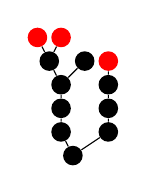
\begin{tikzpicture}[scale=.2]
\node[circle, scale=0.75, fill] (tid0) at (3,1.5){};
\node[circle, scale=0.75, fill] (tid1) at (2.25,3){};
\node[circle, scale=0.75, fill] (tid3) at (2.25,4.5){};
\node[circle, scale=0.75, fill] (tid5) at (2.25,6){};
\node[circle, scale=0.75, fill] (tid7) at (1.5,7.5){};
\node[circle, scale=0.75, fill, red] (tid10) at (0.75,9){};
\node[circle, scale=0.75, fill, red] (tid11) at (2.25,9){};
\draw[](tid7) -- (tid10);
\draw[](tid7) -- (tid11);
\node[circle, scale=0.75, fill] (tid8) at (3.75,7.5){};
\draw[](tid5) -- (tid7);
\draw[](tid5) -- (tid8);
\draw[](tid3) -- (tid5);
\draw[](tid1) -- (tid3);
\node[circle, scale=0.75, fill] (tid2) at (5.25,3){};
\node[circle, scale=0.75, fill] (tid4) at (5.25,4.5){};
\node[circle, scale=0.75, fill] (tid6) at (5.25,6){};
\node[circle, scale=0.75, fill, red] (tid9) at (5.25,7.5){};
\draw[](tid6) -- (tid9);
\draw[](tid4) -- (tid6);
\draw[](tid2) -- (tid4);
\draw[](tid0) -- (tid1);
\draw[](tid0) -- (tid2);
\end{tikzpicture}
\nodepart{two}
\footnotesize{7.25016}
\nodepart{three}
\footnotesize{$33\:67$}
};
 & 
\node[draw=black, rectangle split,  rectangle split parts=3] (sn0x1a11490){
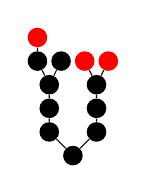
\begin{tikzpicture}[scale=.2]
\node[circle, scale=0.75, fill] (tid0) at (3,1.5){};
\node[circle, scale=0.75, fill] (tid1) at (1.5,3){};
\node[circle, scale=0.75, fill] (tid3) at (1.5,4.5){};
\node[circle, scale=0.75, fill] (tid5) at (1.5,6){};
\node[circle, scale=0.75, fill] (tid7) at (0.75,7.5){};
\node[circle, scale=0.75, fill, red] (tid11) at (0.75,9){};
\draw[](tid7) -- (tid11);
\node[circle, scale=0.75, fill] (tid8) at (2.25,7.5){};
\draw[](tid5) -- (tid7);
\draw[](tid5) -- (tid8);
\draw[](tid3) -- (tid5);
\draw[](tid1) -- (tid3);
\node[circle, scale=0.75, fill] (tid2) at (4.5,3){};
\node[circle, scale=0.75, fill] (tid4) at (4.5,4.5){};
\node[circle, scale=0.75, fill] (tid6) at (4.5,6){};
\node[circle, scale=0.75, fill, red] (tid9) at (3.75,7.5){};
\node[circle, scale=0.75, fill, red] (tid10) at (5.25,7.5){};
\draw[](tid6) -- (tid9);
\draw[](tid6) -- (tid10);
\draw[](tid4) -- (tid6);
\draw[](tid2) -- (tid4);
\draw[](tid0) -- (tid1);
\draw[](tid0) -- (tid2);
\end{tikzpicture}
\nodepart{two}
\footnotesize{7.16582}
\nodepart{three}
\footnotesize{$67\:33$}
};
 & 
\\
};
\end{scope}
\begin{scope}[yshift=\leveltopIII cm]
\matrix (line3) [column sep=1cm] {
\node[draw=black, rectangle split,  rectangle split parts=3] (sn0x1a11800){
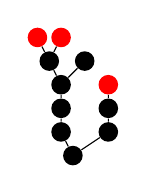
\begin{tikzpicture}[scale=.2]
\node[circle, scale=0.75, fill] (tid0) at (3,1.5){};
\node[circle, scale=0.75, fill] (tid1) at (2.25,3){};
\node[circle, scale=0.75, fill] (tid3) at (2.25,4.5){};
\node[circle, scale=0.75, fill] (tid5) at (2.25,6){};
\node[circle, scale=0.75, fill] (tid7) at (1.5,7.5){};
\node[circle, scale=0.75, fill, red] (tid9) at (0.75,9){};
\node[circle, scale=0.75, fill, red] (tid10) at (2.25,9){};
\draw[](tid7) -- (tid9);
\draw[](tid7) -- (tid10);
\node[circle, scale=0.75, fill] (tid8) at (3.75,7.5){};
\draw[](tid5) -- (tid7);
\draw[](tid5) -- (tid8);
\draw[](tid3) -- (tid5);
\draw[](tid1) -- (tid3);
\node[circle, scale=0.75, fill] (tid2) at (5.25,3){};
\node[circle, scale=0.75, fill] (tid4) at (5.25,4.5){};
\node[circle, scale=0.75, fill, red] (tid6) at (5.25,6){};
\draw[](tid4) -- (tid6);
\draw[](tid2) -- (tid4);
\draw[](tid0) -- (tid1);
\draw[](tid0) -- (tid2);
\end{tikzpicture}
\nodepart{two}
\footnotesize{6.96753}
\nodepart{three}
\footnotesize{$33\:67$}
};
 & 
\node[draw=black, rectangle split,  rectangle split parts=3] (sn0x1a06e70){
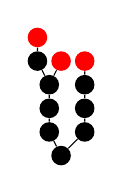
\begin{tikzpicture}[scale=.2]
\node[circle, scale=0.75, fill] (tid0) at (2.25,1.5){};
\node[circle, scale=0.75, fill] (tid1) at (1.5,3){};
\node[circle, scale=0.75, fill] (tid3) at (1.5,4.5){};
\node[circle, scale=0.75, fill] (tid5) at (1.5,6){};
\node[circle, scale=0.75, fill] (tid7) at (0.75,7.5){};
\node[circle, scale=0.75, fill, red] (tid10) at (0.75,9){};
\draw[](tid7) -- (tid10);
\node[circle, scale=0.75, fill, red] (tid8) at (2.25,7.5){};
\draw[](tid5) -- (tid7);
\draw[](tid5) -- (tid8);
\draw[](tid3) -- (tid5);
\draw[](tid1) -- (tid3);
\node[circle, scale=0.75, fill] (tid2) at (3.75,3){};
\node[circle, scale=0.75, fill] (tid4) at (3.75,4.5){};
\node[circle, scale=0.75, fill] (tid6) at (3.75,6){};
\node[circle, scale=0.75, fill, red] (tid9) at (3.75,7.5){};
\draw[](tid6) -- (tid9);
\draw[](tid4) -- (tid6);
\draw[](tid2) -- (tid4);
\draw[](tid0) -- (tid1);
\draw[](tid0) -- (tid2);
\end{tikzpicture}
\nodepart{two}
\footnotesize{6.89148}
\nodepart{three}
\footnotesize{$33\:33\:33$}
};
 & 
\node[draw=black, rectangle split,  rectangle split parts=3] (sn0x1a09570){
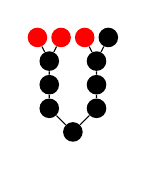
\begin{tikzpicture}[scale=.2]
\node[circle, scale=0.75, fill] (tid0) at (3,1.5){};
\node[circle, scale=0.75, fill] (tid1) at (1.5,3){};
\node[circle, scale=0.75, fill] (tid3) at (1.5,4.5){};
\node[circle, scale=0.75, fill] (tid5) at (1.5,6){};
\node[circle, scale=0.75, fill, red] (tid7) at (0.75,7.5){};
\node[circle, scale=0.75, fill, red] (tid8) at (2.25,7.5){};
\draw[](tid5) -- (tid7);
\draw[](tid5) -- (tid8);
\draw[](tid3) -- (tid5);
\draw[](tid1) -- (tid3);
\node[circle, scale=0.75, fill] (tid2) at (4.5,3){};
\node[circle, scale=0.75, fill] (tid4) at (4.5,4.5){};
\node[circle, scale=0.75, fill] (tid6) at (4.5,6){};
\node[circle, scale=0.75, fill, red] (tid9) at (3.75,7.5){};
\node[circle, scale=0.75, fill] (tid10) at (5.25,7.5){};
\draw[](tid6) -- (tid9);
\draw[](tid6) -- (tid10);
\draw[](tid4) -- (tid6);
\draw[](tid2) -- (tid4);
\draw[](tid0) -- (tid1);
\draw[](tid0) -- (tid2);
\end{tikzpicture}
\nodepart{two}
\footnotesize{6.71451}
\nodepart{three}
\footnotesize{$1$}
};
 & 
\\
};
\end{scope}
\begin{scope}[yshift=\leveltopIIII cm]
\matrix (line4) [column sep=1cm] {
\node[draw=black, rectangle split,  rectangle split parts=3] (sn0x1a0d820){
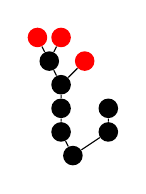
\begin{tikzpicture}[scale=.2]
\node[circle, scale=0.75, fill] (tid0) at (3,1.5){};
\node[circle, scale=0.75, fill] (tid1) at (2.25,3){};
\node[circle, scale=0.75, fill] (tid3) at (2.25,4.5){};
\node[circle, scale=0.75, fill] (tid5) at (2.25,6){};
\node[circle, scale=0.75, fill] (tid6) at (1.5,7.5){};
\node[circle, scale=0.75, fill, red] (tid8) at (0.75,9){};
\node[circle, scale=0.75, fill, red] (tid9) at (2.25,9){};
\draw[](tid6) -- (tid8);
\draw[](tid6) -- (tid9);
\node[circle, scale=0.75, fill, red] (tid7) at (3.75,7.5){};
\draw[](tid5) -- (tid6);
\draw[](tid5) -- (tid7);
\draw[](tid3) -- (tid5);
\draw[](tid1) -- (tid3);
\node[circle, scale=0.75, fill] (tid2) at (5.25,3){};
\node[circle, scale=0.75, fill] (tid4) at (5.25,4.5){};
\draw[](tid2) -- (tid4);
\draw[](tid0) -- (tid1);
\draw[](tid0) -- (tid2);
\end{tikzpicture}
\nodepart{two}
\footnotesize{6.77701}
\nodepart{three}
\footnotesize{$33\:67$}
};
 & 
\node[draw=black, rectangle split,  rectangle split parts=3] (sn0x1a09090){
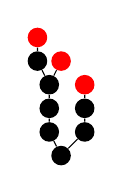
\begin{tikzpicture}[scale=.2]
\node[circle, scale=0.75, fill] (tid0) at (2.25,1.5){};
\node[circle, scale=0.75, fill] (tid1) at (1.5,3){};
\node[circle, scale=0.75, fill] (tid3) at (1.5,4.5){};
\node[circle, scale=0.75, fill] (tid5) at (1.5,6){};
\node[circle, scale=0.75, fill] (tid7) at (0.75,7.5){};
\node[circle, scale=0.75, fill, red] (tid9) at (0.75,9){};
\draw[](tid7) -- (tid9);
\node[circle, scale=0.75, fill, red] (tid8) at (2.25,7.5){};
\draw[](tid5) -- (tid7);
\draw[](tid5) -- (tid8);
\draw[](tid3) -- (tid5);
\draw[](tid1) -- (tid3);
\node[circle, scale=0.75, fill] (tid2) at (3.75,3){};
\node[circle, scale=0.75, fill] (tid4) at (3.75,4.5){};
\node[circle, scale=0.75, fill, red] (tid6) at (3.75,6){};
\draw[](tid4) -- (tid6);
\draw[](tid2) -- (tid4);
\draw[](tid0) -- (tid1);
\draw[](tid0) -- (tid2);
\end{tikzpicture}
\nodepart{two}
\footnotesize{6.56279}
\nodepart{three}
\footnotesize{$33\:33\:33$}
};
 & 
\node[draw=black, rectangle split,  rectangle split parts=3] (sn0x1a039e0){
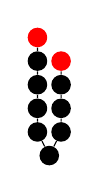
\begin{tikzpicture}[scale=.2]
\node[circle, scale=0.75, fill] (tid0) at (1.5,1.5){};
\node[circle, scale=0.75, fill] (tid1) at (0.75,3){};
\node[circle, scale=0.75, fill] (tid3) at (0.75,4.5){};
\node[circle, scale=0.75, fill] (tid5) at (0.75,6){};
\node[circle, scale=0.75, fill] (tid7) at (0.75,7.5){};
\node[circle, scale=0.75, fill, red] (tid9) at (0.75,9){};
\draw[](tid7) -- (tid9);
\draw[](tid5) -- (tid7);
\draw[](tid3) -- (tid5);
\draw[](tid1) -- (tid3);
\node[circle, scale=0.75, fill] (tid2) at (2.25,3){};
\node[circle, scale=0.75, fill] (tid4) at (2.25,4.5){};
\node[circle, scale=0.75, fill] (tid6) at (2.25,6){};
\node[circle, scale=0.75, fill, red] (tid8) at (2.25,7.5){};
\draw[](tid6) -- (tid8);
\draw[](tid4) -- (tid6);
\draw[](tid2) -- (tid4);
\draw[](tid0) -- (tid1);
\draw[](tid0) -- (tid2);
\end{tikzpicture}
\nodepart{two}
\footnotesize{6.73047}
\nodepart{three}
\footnotesize{$50\:50$}
};
 & 
\node[draw=black, rectangle split,  rectangle split parts=3] (sn0x1a068a0){
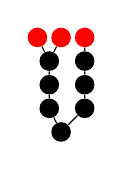
\begin{tikzpicture}[scale=.2]
\node[circle, scale=0.75, fill] (tid0) at (2.25,1.5){};
\node[circle, scale=0.75, fill] (tid1) at (1.5,3){};
\node[circle, scale=0.75, fill] (tid3) at (1.5,4.5){};
\node[circle, scale=0.75, fill] (tid5) at (1.5,6){};
\node[circle, scale=0.75, fill, red] (tid7) at (0.75,7.5){};
\node[circle, scale=0.75, fill, red] (tid8) at (2.25,7.5){};
\draw[](tid5) -- (tid7);
\draw[](tid5) -- (tid8);
\draw[](tid3) -- (tid5);
\draw[](tid1) -- (tid3);
\node[circle, scale=0.75, fill] (tid2) at (3.75,3){};
\node[circle, scale=0.75, fill] (tid4) at (3.75,4.5){};
\node[circle, scale=0.75, fill] (tid6) at (3.75,6){};
\node[circle, scale=0.75, fill, red] (tid9) at (3.75,7.5){};
\draw[](tid6) -- (tid9);
\draw[](tid4) -- (tid6);
\draw[](tid2) -- (tid4);
\draw[](tid0) -- (tid1);
\draw[](tid0) -- (tid2);
\end{tikzpicture}
\nodepart{two}
\footnotesize{6.38117}
\nodepart{three}
\footnotesize{$33\:67$}
};
 & 
\\
};
\end{scope}
\begin{scope}[yshift=\leveltopIIIII cm]
\matrix (line5) [column sep=1cm] {
\node[draw=black, rectangle split,  rectangle split parts=3] (sn0x1a01a50){
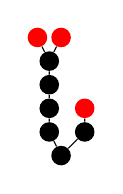
\begin{tikzpicture}[scale=.2]
\node[circle, scale=0.75, fill] (tid0) at (2.25,1.5){};
\node[circle, scale=0.75, fill] (tid1) at (1.5,3){};
\node[circle, scale=0.75, fill] (tid3) at (1.5,4.5){};
\node[circle, scale=0.75, fill] (tid5) at (1.5,6){};
\node[circle, scale=0.75, fill] (tid6) at (1.5,7.5){};
\node[circle, scale=0.75, fill, red] (tid7) at (0.75,9){};
\node[circle, scale=0.75, fill, red] (tid8) at (2.25,9){};
\draw[](tid6) -- (tid7);
\draw[](tid6) -- (tid8);
\draw[](tid5) -- (tid6);
\draw[](tid3) -- (tid5);
\draw[](tid1) -- (tid3);
\node[circle, scale=0.75, fill] (tid2) at (3.75,3){};
\node[circle, scale=0.75, fill, red] (tid4) at (3.75,4.5){};
\draw[](tid2) -- (tid4);
\draw[](tid0) -- (tid1);
\draw[](tid0) -- (tid2);
\end{tikzpicture}
\nodepart{two}
\footnotesize{6.60069}
\nodepart{three}
\footnotesize{$33\:67$}
};
 & 
\node[draw=black, rectangle split,  rectangle split parts=3] (sn0x1a08e90){
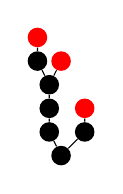
\begin{tikzpicture}[scale=.2]
\node[circle, scale=0.75, fill] (tid0) at (2.25,1.5){};
\node[circle, scale=0.75, fill] (tid1) at (1.5,3){};
\node[circle, scale=0.75, fill] (tid3) at (1.5,4.5){};
\node[circle, scale=0.75, fill] (tid5) at (1.5,6){};
\node[circle, scale=0.75, fill] (tid6) at (0.75,7.5){};
\node[circle, scale=0.75, fill, red] (tid8) at (0.75,9){};
\draw[](tid6) -- (tid8);
\node[circle, scale=0.75, fill, red] (tid7) at (2.25,7.5){};
\draw[](tid5) -- (tid6);
\draw[](tid5) -- (tid7);
\draw[](tid3) -- (tid5);
\draw[](tid1) -- (tid3);
\node[circle, scale=0.75, fill] (tid2) at (3.75,3){};
\node[circle, scale=0.75, fill, red] (tid4) at (3.75,4.5){};
\draw[](tid2) -- (tid4);
\draw[](tid0) -- (tid1);
\draw[](tid0) -- (tid2);
\end{tikzpicture}
\nodepart{two}
\footnotesize{6.36516}
\nodepart{three}
\footnotesize{$33\:33\:33$}
};
 & 
\node[draw=black, rectangle split,  rectangle split parts=3] (sn0x1a02f80){
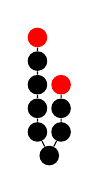
\begin{tikzpicture}[scale=.2]
\node[circle, scale=0.75, fill] (tid0) at (1.5,1.5){};
\node[circle, scale=0.75, fill] (tid1) at (0.75,3){};
\node[circle, scale=0.75, fill] (tid3) at (0.75,4.5){};
\node[circle, scale=0.75, fill] (tid5) at (0.75,6){};
\node[circle, scale=0.75, fill] (tid7) at (0.75,7.5){};
\node[circle, scale=0.75, fill, red] (tid8) at (0.75,9){};
\draw[](tid7) -- (tid8);
\draw[](tid5) -- (tid7);
\draw[](tid3) -- (tid5);
\draw[](tid1) -- (tid3);
\node[circle, scale=0.75, fill] (tid2) at (2.25,3){};
\node[circle, scale=0.75, fill] (tid4) at (2.25,4.5){};
\node[circle, scale=0.75, fill, red] (tid6) at (2.25,6){};
\draw[](tid4) -- (tid6);
\draw[](tid2) -- (tid4);
\draw[](tid0) -- (tid1);
\draw[](tid0) -- (tid2);
\end{tikzpicture}
\nodepart{two}
\footnotesize{6.36719}
\nodepart{three}
\footnotesize{$50\:50$}
};
 & 
\node[draw=black, rectangle split,  rectangle split parts=3] (sn0x1a064f0){
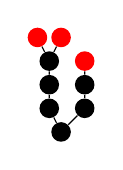
\begin{tikzpicture}[scale=.2]
\node[circle, scale=0.75, fill] (tid0) at (2.25,1.5){};
\node[circle, scale=0.75, fill] (tid1) at (1.5,3){};
\node[circle, scale=0.75, fill] (tid3) at (1.5,4.5){};
\node[circle, scale=0.75, fill] (tid5) at (1.5,6){};
\node[circle, scale=0.75, fill, red] (tid7) at (0.75,7.5){};
\node[circle, scale=0.75, fill, red] (tid8) at (2.25,7.5){};
\draw[](tid5) -- (tid7);
\draw[](tid5) -- (tid8);
\draw[](tid3) -- (tid5);
\draw[](tid1) -- (tid3);
\node[circle, scale=0.75, fill] (tid2) at (3.75,3){};
\node[circle, scale=0.75, fill] (tid4) at (3.75,4.5){};
\node[circle, scale=0.75, fill, red] (tid6) at (3.75,6){};
\draw[](tid4) -- (tid6);
\draw[](tid2) -- (tid4);
\draw[](tid0) -- (tid1);
\draw[](tid0) -- (tid2);
\end{tikzpicture}
\nodepart{two}
\footnotesize{5.95602}
\nodepart{three}
\footnotesize{$33\:67$}
};
 & 
\node[draw=black, rectangle split,  rectangle split parts=3] (sn0x1a03650){
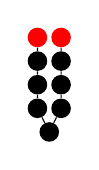
\begin{tikzpicture}[scale=.2]
\node[circle, scale=0.75, fill] (tid0) at (1.5,1.5){};
\node[circle, scale=0.75, fill] (tid1) at (0.75,3){};
\node[circle, scale=0.75, fill] (tid3) at (0.75,4.5){};
\node[circle, scale=0.75, fill] (tid5) at (0.75,6){};
\node[circle, scale=0.75, fill, red] (tid7) at (0.75,7.5){};
\draw[](tid5) -- (tid7);
\draw[](tid3) -- (tid5);
\draw[](tid1) -- (tid3);
\node[circle, scale=0.75, fill] (tid2) at (2.25,3){};
\node[circle, scale=0.75, fill] (tid4) at (2.25,4.5){};
\node[circle, scale=0.75, fill] (tid6) at (2.25,6){};
\node[circle, scale=0.75, fill, red] (tid8) at (2.25,7.5){};
\draw[](tid6) -- (tid8);
\draw[](tid4) -- (tid6);
\draw[](tid2) -- (tid4);
\draw[](tid0) -- (tid1);
\draw[](tid0) -- (tid2);
\end{tikzpicture}
\nodepart{two}
\footnotesize{6.09375}
\nodepart{three}
\footnotesize{$1$}
};
 & 
\\
};
\end{scope}
\begin{scope}[yshift=\leveltopIIIIII cm]
\matrix (line6) [column sep=1cm] {
\node[draw=black, rectangle split,  rectangle split parts=3] (sn0x1a00320){
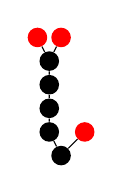
\begin{tikzpicture}[scale=.2]
\node[circle, scale=0.75, fill] (tid0) at (2.25,1.5){};
\node[circle, scale=0.75, fill] (tid1) at (1.5,3){};
\node[circle, scale=0.75, fill] (tid3) at (1.5,4.5){};
\node[circle, scale=0.75, fill] (tid4) at (1.5,6){};
\node[circle, scale=0.75, fill] (tid5) at (1.5,7.5){};
\node[circle, scale=0.75, fill, red] (tid6) at (0.75,9){};
\node[circle, scale=0.75, fill, red] (tid7) at (2.25,9){};
\draw[](tid5) -- (tid6);
\draw[](tid5) -- (tid7);
\draw[](tid4) -- (tid5);
\draw[](tid3) -- (tid4);
\draw[](tid1) -- (tid3);
\node[circle, scale=0.75, fill, red] (tid2) at (3.75,3){};
\draw[](tid0) -- (tid1);
\draw[](tid0) -- (tid2);
\end{tikzpicture}
\nodepart{two}
\footnotesize{6.52083}
\nodepart{three}
\footnotesize{$33\:67$}
};
 & 
\node[draw=black, rectangle split,  rectangle split parts=3] (sn0x1a01980){
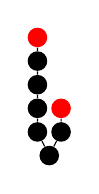
\begin{tikzpicture}[scale=.2]
\node[circle, scale=0.75, fill] (tid0) at (1.5,1.5){};
\node[circle, scale=0.75, fill] (tid1) at (0.75,3){};
\node[circle, scale=0.75, fill] (tid3) at (0.75,4.5){};
\node[circle, scale=0.75, fill] (tid5) at (0.75,6){};
\node[circle, scale=0.75, fill] (tid6) at (0.75,7.5){};
\node[circle, scale=0.75, fill, red] (tid7) at (0.75,9){};
\draw[](tid6) -- (tid7);
\draw[](tid5) -- (tid6);
\draw[](tid3) -- (tid5);
\draw[](tid1) -- (tid3);
\node[circle, scale=0.75, fill] (tid2) at (2.25,3){};
\node[circle, scale=0.75, fill, red] (tid4) at (2.25,4.5){};
\draw[](tid2) -- (tid4);
\draw[](tid0) -- (tid1);
\draw[](tid0) -- (tid2);
\end{tikzpicture}
\nodepart{two}
\footnotesize{6.14062}
\nodepart{three}
\footnotesize{$50\:50$}
};
 & 
\node[draw=black, rectangle split,  rectangle split parts=3] (sn0x1a08dc0){
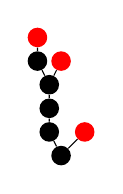
\begin{tikzpicture}[scale=.2]
\node[circle, scale=0.75, fill] (tid0) at (2.25,1.5){};
\node[circle, scale=0.75, fill] (tid1) at (1.5,3){};
\node[circle, scale=0.75, fill] (tid3) at (1.5,4.5){};
\node[circle, scale=0.75, fill] (tid4) at (1.5,6){};
\node[circle, scale=0.75, fill] (tid5) at (0.75,7.5){};
\node[circle, scale=0.75, fill, red] (tid7) at (0.75,9){};
\draw[](tid5) -- (tid7);
\node[circle, scale=0.75, fill, red] (tid6) at (2.25,7.5){};
\draw[](tid4) -- (tid5);
\draw[](tid4) -- (tid6);
\draw[](tid3) -- (tid4);
\draw[](tid1) -- (tid3);
\node[circle, scale=0.75, fill, red] (tid2) at (3.75,3){};
\draw[](tid0) -- (tid1);
\draw[](tid0) -- (tid2);
\end{tikzpicture}
\nodepart{two}
\footnotesize{6.27431}
\nodepart{three}
\footnotesize{$33\:33\:33$}
};
 & 
\node[draw=black, rectangle split,  rectangle split parts=3] (sn0x1a06420){
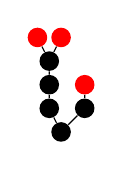
\begin{tikzpicture}[scale=.2]
\node[circle, scale=0.75, fill] (tid0) at (2.25,1.5){};
\node[circle, scale=0.75, fill] (tid1) at (1.5,3){};
\node[circle, scale=0.75, fill] (tid3) at (1.5,4.5){};
\node[circle, scale=0.75, fill] (tid5) at (1.5,6){};
\node[circle, scale=0.75, fill, red] (tid6) at (0.75,7.5){};
\node[circle, scale=0.75, fill, red] (tid7) at (2.25,7.5){};
\draw[](tid5) -- (tid6);
\draw[](tid5) -- (tid7);
\draw[](tid3) -- (tid5);
\draw[](tid1) -- (tid3);
\node[circle, scale=0.75, fill] (tid2) at (3.75,3){};
\node[circle, scale=0.75, fill, red] (tid4) at (3.75,4.5){};
\draw[](tid2) -- (tid4);
\draw[](tid0) -- (tid1);
\draw[](tid0) -- (tid2);
\end{tikzpicture}
\nodepart{two}
\footnotesize{5.68056}
\nodepart{three}
\footnotesize{$67\:33$}
};
 & 
\node[draw=black, rectangle split,  rectangle split parts=3] (sn0x1a02160){
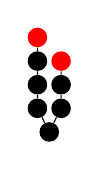
\begin{tikzpicture}[scale=.2]
\node[circle, scale=0.75, fill] (tid0) at (1.5,1.5){};
\node[circle, scale=0.75, fill] (tid1) at (0.75,3){};
\node[circle, scale=0.75, fill] (tid3) at (0.75,4.5){};
\node[circle, scale=0.75, fill] (tid5) at (0.75,6){};
\node[circle, scale=0.75, fill, red] (tid7) at (0.75,7.5){};
\draw[](tid5) -- (tid7);
\draw[](tid3) -- (tid5);
\draw[](tid1) -- (tid3);
\node[circle, scale=0.75, fill] (tid2) at (2.25,3){};
\node[circle, scale=0.75, fill] (tid4) at (2.25,4.5){};
\node[circle, scale=0.75, fill, red] (tid6) at (2.25,6){};
\draw[](tid4) -- (tid6);
\draw[](tid2) -- (tid4);
\draw[](tid0) -- (tid1);
\draw[](tid0) -- (tid2);
\end{tikzpicture}
\nodepart{two}
\footnotesize{5.59375}
\nodepart{three}
\footnotesize{$50\:50$}
};
 & 
\\
};
\end{scope}
\begin{scope}[yshift=\leveltopIIIIIII cm]
\matrix (line7) [column sep=1cm] {
\node[draw=black, rectangle split,  rectangle split parts=3] (sn0x19feaa0){
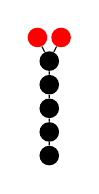
\begin{tikzpicture}[scale=.2]
\node[circle, scale=0.75, fill] (tid0) at (1.5,1.5){};
\node[circle, scale=0.75, fill] (tid1) at (1.5,3){};
\node[circle, scale=0.75, fill] (tid2) at (1.5,4.5){};
\node[circle, scale=0.75, fill] (tid3) at (1.5,6){};
\node[circle, scale=0.75, fill] (tid4) at (1.5,7.5){};
\node[circle, scale=0.75, fill, red] (tid5) at (0.75,9){};
\node[circle, scale=0.75, fill, red] (tid6) at (2.25,9){};
\draw[](tid4) -- (tid5);
\draw[](tid4) -- (tid6);
\draw[](tid3) -- (tid4);
\draw[](tid2) -- (tid3);
\draw[](tid1) -- (tid2);
\draw[](tid0) -- (tid1);
\end{tikzpicture}
\nodepart{two}
\footnotesize{6.5}
\nodepart{three}
\footnotesize{$1$}
};
 & 
\node[draw=black, rectangle split,  rectangle split parts=3] (sn0x1a00090){
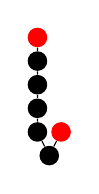
\begin{tikzpicture}[scale=.2]
\node[circle, scale=0.75, fill] (tid0) at (1.5,1.5){};
\node[circle, scale=0.75, fill] (tid1) at (0.75,3){};
\node[circle, scale=0.75, fill] (tid3) at (0.75,4.5){};
\node[circle, scale=0.75, fill] (tid4) at (0.75,6){};
\node[circle, scale=0.75, fill] (tid5) at (0.75,7.5){};
\node[circle, scale=0.75, fill, red] (tid6) at (0.75,9){};
\draw[](tid5) -- (tid6);
\draw[](tid4) -- (tid5);
\draw[](tid3) -- (tid4);
\draw[](tid1) -- (tid3);
\node[circle, scale=0.75, fill, red] (tid2) at (2.25,3){};
\draw[](tid0) -- (tid1);
\draw[](tid0) -- (tid2);
\end{tikzpicture}
\nodepart{two}
\footnotesize{6.03125}
\nodepart{three}
\footnotesize{$50\:50$}
};
 & 
\node[draw=black, rectangle split,  rectangle split parts=3] (sn0x1a01760){
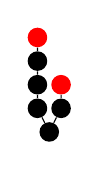
\begin{tikzpicture}[scale=.2]
\node[circle, scale=0.75, fill] (tid0) at (1.5,1.5){};
\node[circle, scale=0.75, fill] (tid1) at (0.75,3){};
\node[circle, scale=0.75, fill] (tid3) at (0.75,4.5){};
\node[circle, scale=0.75, fill] (tid5) at (0.75,6){};
\node[circle, scale=0.75, fill, red] (tid6) at (0.75,7.5){};
\draw[](tid5) -- (tid6);
\draw[](tid3) -- (tid5);
\draw[](tid1) -- (tid3);
\node[circle, scale=0.75, fill] (tid2) at (2.25,3){};
\node[circle, scale=0.75, fill, red] (tid4) at (2.25,4.5){};
\draw[](tid2) -- (tid4);
\draw[](tid0) -- (tid1);
\draw[](tid0) -- (tid2);
\end{tikzpicture}
\nodepart{two}
\footnotesize{5.25}
\nodepart{three}
\footnotesize{$50\:50$}
};
 & 
\node[draw=black, rectangle split,  rectangle split parts=3] (sn0x1a07c30){
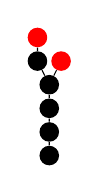
\begin{tikzpicture}[scale=.2]
\node[circle, scale=0.75, fill] (tid0) at (1.5,1.5){};
\node[circle, scale=0.75, fill] (tid1) at (1.5,3){};
\node[circle, scale=0.75, fill] (tid2) at (1.5,4.5){};
\node[circle, scale=0.75, fill] (tid3) at (1.5,6){};
\node[circle, scale=0.75, fill] (tid4) at (0.75,7.5){};
\node[circle, scale=0.75, fill, red] (tid6) at (0.75,9){};
\draw[](tid4) -- (tid6);
\node[circle, scale=0.75, fill, red] (tid5) at (2.25,7.5){};
\draw[](tid3) -- (tid4);
\draw[](tid3) -- (tid5);
\draw[](tid2) -- (tid3);
\draw[](tid1) -- (tid2);
\draw[](tid0) -- (tid1);
\end{tikzpicture}
\nodepart{two}
\footnotesize{6.25}
\nodepart{three}
\footnotesize{$50\:50$}
};
 & 
\node[draw=black, rectangle split,  rectangle split parts=3] (sn0x1a04ed0){
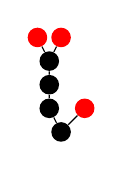
\begin{tikzpicture}[scale=.2]
\node[circle, scale=0.75, fill] (tid0) at (2.25,1.5){};
\node[circle, scale=0.75, fill] (tid1) at (1.5,3){};
\node[circle, scale=0.75, fill] (tid3) at (1.5,4.5){};
\node[circle, scale=0.75, fill] (tid4) at (1.5,6){};
\node[circle, scale=0.75, fill, red] (tid5) at (0.75,7.5){};
\node[circle, scale=0.75, fill, red] (tid6) at (2.25,7.5){};
\draw[](tid4) -- (tid5);
\draw[](tid4) -- (tid6);
\draw[](tid3) -- (tid4);
\draw[](tid1) -- (tid3);
\node[circle, scale=0.75, fill, red] (tid2) at (3.75,3){};
\draw[](tid0) -- (tid1);
\draw[](tid0) -- (tid2);
\end{tikzpicture}
\nodepart{two}
\footnotesize{5.54167}
\nodepart{three}
\footnotesize{$67\:33$}
};
 & 
\node[draw=black, rectangle split,  rectangle split parts=3] (sn0x1a02050){
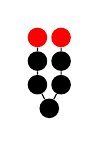
\begin{tikzpicture}[scale=.2]
\node[circle, scale=0.75, fill] (tid0) at (1.5,1.5){};
\node[circle, scale=0.75, fill] (tid1) at (0.75,3){};
\node[circle, scale=0.75, fill] (tid3) at (0.75,4.5){};
\node[circle, scale=0.75, fill, red] (tid5) at (0.75,6){};
\draw[](tid3) -- (tid5);
\draw[](tid1) -- (tid3);
\node[circle, scale=0.75, fill] (tid2) at (2.25,3){};
\node[circle, scale=0.75, fill] (tid4) at (2.25,4.5){};
\node[circle, scale=0.75, fill, red] (tid6) at (2.25,6){};
\draw[](tid4) -- (tid6);
\draw[](tid2) -- (tid4);
\draw[](tid0) -- (tid1);
\draw[](tid0) -- (tid2);
\end{tikzpicture}
\nodepart{two}
\footnotesize{4.9375}
\nodepart{three}
\footnotesize{$1$}
};
 & 
\\
};
\end{scope}
\begin{scope}[yshift=\leveltopIIIIIIII cm]
\matrix (line8) [column sep=1cm] {
\node[draw=black, rectangle split,  rectangle split parts=3] (sn0x19fe9d0){
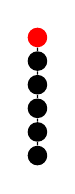
\begin{tikzpicture}[scale=.2]
\node[circle, scale=0.75, fill] (tid0) at (0.75,1.5){};
\node[circle, scale=0.75, fill] (tid1) at (0.75,3){};
\node[circle, scale=0.75, fill] (tid2) at (0.75,4.5){};
\node[circle, scale=0.75, fill] (tid3) at (0.75,6){};
\node[circle, scale=0.75, fill] (tid4) at (0.75,7.5){};
\node[circle, scale=0.75, fill, red] (tid5) at (0.75,9){};
\draw[](tid4) -- (tid5);
\draw[](tid3) -- (tid4);
\draw[](tid2) -- (tid3);
\draw[](tid1) -- (tid2);
\draw[](tid0) -- (tid1);
\end{tikzpicture}
\nodepart{two}
\footnotesize{6}
\nodepart{three}
\footnotesize{$1$}
};
 & 
\node[draw=black, rectangle split,  rectangle split parts=3] (sn0x19ffef0){
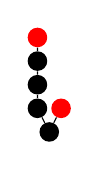
\begin{tikzpicture}[scale=.2]
\node[circle, scale=0.75, fill] (tid0) at (1.5,1.5){};
\node[circle, scale=0.75, fill] (tid1) at (0.75,3){};
\node[circle, scale=0.75, fill] (tid3) at (0.75,4.5){};
\node[circle, scale=0.75, fill] (tid4) at (0.75,6){};
\node[circle, scale=0.75, fill, red] (tid5) at (0.75,7.5){};
\draw[](tid4) -- (tid5);
\draw[](tid3) -- (tid4);
\draw[](tid1) -- (tid3);
\node[circle, scale=0.75, fill, red] (tid2) at (2.25,3){};
\draw[](tid0) -- (tid1);
\draw[](tid0) -- (tid2);
\end{tikzpicture}
\nodepart{two}
\footnotesize{5.0625}
\nodepart{three}
\footnotesize{$50\:50$}
};
 & 
\node[draw=black, rectangle split,  rectangle split parts=3] (sn0x1a008c0){
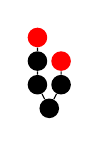
\begin{tikzpicture}[scale=.2]
\node[circle, scale=0.75, fill] (tid0) at (1.5,1.5){};
\node[circle, scale=0.75, fill] (tid1) at (0.75,3){};
\node[circle, scale=0.75, fill] (tid3) at (0.75,4.5){};
\node[circle, scale=0.75, fill, red] (tid5) at (0.75,6){};
\draw[](tid3) -- (tid5);
\draw[](tid1) -- (tid3);
\node[circle, scale=0.75, fill] (tid2) at (2.25,3){};
\node[circle, scale=0.75, fill, red] (tid4) at (2.25,4.5){};
\draw[](tid2) -- (tid4);
\draw[](tid0) -- (tid1);
\draw[](tid0) -- (tid2);
\end{tikzpicture}
\nodepart{two}
\footnotesize{4.4375}
\nodepart{three}
\footnotesize{$50\:50$}
};
 & 
\node[draw=black, rectangle split,  rectangle split parts=3] (sn0x1a06160){
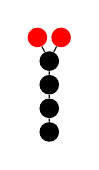
\begin{tikzpicture}[scale=.2]
\node[circle, scale=0.75, fill] (tid0) at (1.5,1.5){};
\node[circle, scale=0.75, fill] (tid1) at (1.5,3){};
\node[circle, scale=0.75, fill] (tid2) at (1.5,4.5){};
\node[circle, scale=0.75, fill] (tid3) at (1.5,6){};
\node[circle, scale=0.75, fill, red] (tid4) at (0.75,7.5){};
\node[circle, scale=0.75, fill, red] (tid5) at (2.25,7.5){};
\draw[](tid3) -- (tid4);
\draw[](tid3) -- (tid5);
\draw[](tid2) -- (tid3);
\draw[](tid1) -- (tid2);
\draw[](tid0) -- (tid1);
\end{tikzpicture}
\nodepart{two}
\footnotesize{5.5}
\nodepart{three}
\footnotesize{$1$}
};
 & 
\\
};
\end{scope}
\begin{scope}[yshift=\leveltopIIIIIIIII cm]
\matrix (line9) [column sep=1cm] {
\node[draw=black, rectangle split,  rectangle split parts=3] (sn0x19fe430){
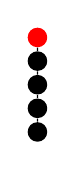
\begin{tikzpicture}[scale=.2]
\node[circle, scale=0.75, fill] (tid0) at (0.75,1.5){};
\node[circle, scale=0.75, fill] (tid1) at (0.75,3){};
\node[circle, scale=0.75, fill] (tid2) at (0.75,4.5){};
\node[circle, scale=0.75, fill] (tid3) at (0.75,6){};
\node[circle, scale=0.75, fill, red] (tid4) at (0.75,7.5){};
\draw[](tid3) -- (tid4);
\draw[](tid2) -- (tid3);
\draw[](tid1) -- (tid2);
\draw[](tid0) -- (tid1);
\end{tikzpicture}
\nodepart{two}
\footnotesize{5}
\nodepart{three}
\footnotesize{$1$}
};
 & 
\node[draw=black, rectangle split,  rectangle split parts=3] (sn0x19ffa30){
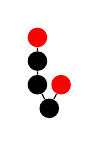
\begin{tikzpicture}[scale=.2]
\node[circle, scale=0.75, fill] (tid0) at (1.5,1.5){};
\node[circle, scale=0.75, fill] (tid1) at (0.75,3){};
\node[circle, scale=0.75, fill] (tid3) at (0.75,4.5){};
\node[circle, scale=0.75, fill, red] (tid4) at (0.75,6){};
\draw[](tid3) -- (tid4);
\draw[](tid1) -- (tid3);
\node[circle, scale=0.75, fill, red] (tid2) at (2.25,3){};
\draw[](tid0) -- (tid1);
\draw[](tid0) -- (tid2);
\end{tikzpicture}
\nodepart{two}
\footnotesize{4.125}
\nodepart{three}
\footnotesize{$50\:50$}
};
 & 
\node[draw=black, rectangle split,  rectangle split parts=3] (sn0x1a007d0){
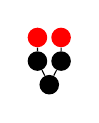
\begin{tikzpicture}[scale=.2]
\node[circle, scale=0.75, fill] (tid0) at (1.5,1.5){};
\node[circle, scale=0.75, fill] (tid1) at (0.75,3){};
\node[circle, scale=0.75, fill, red] (tid3) at (0.75,4.5){};
\draw[](tid1) -- (tid3);
\node[circle, scale=0.75, fill] (tid2) at (2.25,3){};
\node[circle, scale=0.75, fill, red] (tid4) at (2.25,4.5){};
\draw[](tid2) -- (tid4);
\draw[](tid0) -- (tid1);
\draw[](tid0) -- (tid2);
\end{tikzpicture}
\nodepart{two}
\footnotesize{3.75}
\nodepart{three}
\footnotesize{$1$}
};
 & 
\\
};
\end{scope}
\begin{scope}[yshift=\leveltopIIIIIIIIII cm]
\matrix (line10) [column sep=1cm] {
\node[draw=black, rectangle split,  rectangle split parts=3] (sn0x19fe300){
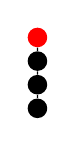
\begin{tikzpicture}[scale=.2]
\node[circle, scale=0.75, fill] (tid0) at (0.75,1.5){};
\node[circle, scale=0.75, fill] (tid1) at (0.75,3){};
\node[circle, scale=0.75, fill] (tid2) at (0.75,4.5){};
\node[circle, scale=0.75, fill, red] (tid3) at (0.75,6){};
\draw[](tid2) -- (tid3);
\draw[](tid1) -- (tid2);
\draw[](tid0) -- (tid1);
\end{tikzpicture}
\nodepart{two}
\footnotesize{4}
\nodepart{three}
\footnotesize{$1$}
};
 & 
\node[draw=black, rectangle split,  rectangle split parts=3] (sn0x19fedf0){
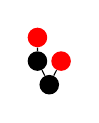
\begin{tikzpicture}[scale=.2]
\node[circle, scale=0.75, fill] (tid0) at (1.5,1.5){};
\node[circle, scale=0.75, fill] (tid1) at (0.75,3){};
\node[circle, scale=0.75, fill, red] (tid3) at (0.75,4.5){};
\draw[](tid1) -- (tid3);
\node[circle, scale=0.75, fill, red] (tid2) at (2.25,3){};
\draw[](tid0) -- (tid1);
\draw[](tid0) -- (tid2);
\end{tikzpicture}
\nodepart{two}
\footnotesize{3.25}
\nodepart{three}
\footnotesize{$50\:50$}
};
 & 
\\
};
\end{scope}
\begin{scope}[yshift=\leveltopIIIIIIIIIII cm]
\matrix (line11) [column sep=1cm] {
\node[draw=black, rectangle split,  rectangle split parts=3] (sn0x19fe230){
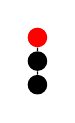
\begin{tikzpicture}[scale=.2]
\node[circle, scale=0.75, fill] (tid0) at (0.75,1.5){};
\node[circle, scale=0.75, fill] (tid1) at (0.75,3){};
\node[circle, scale=0.75, fill, red] (tid2) at (0.75,4.5){};
\draw[](tid1) -- (tid2);
\draw[](tid0) -- (tid1);
\end{tikzpicture}
\nodepart{two}
\footnotesize{3}
\nodepart{three}
\footnotesize{$1$}
};
 & 
\node[draw=black, rectangle split,  rectangle split parts=3] (sn0x19fed20){

\begin{tikzpicture}[scale=.2]
\node[circle, scale=0.75, fill] (tid0) at (1.5,1.5){};
\node[circle, scale=0.75, fill, red] (tid1) at (0.75,3){};
\node[circle, scale=0.75, fill, red] (tid2) at (2.25,3){};
\draw[](tid0) -- (tid1);
\draw[](tid0) -- (tid2);
\end{tikzpicture}
\nodepart{two}
\footnotesize{2.5}
\nodepart{three}
\footnotesize{$1$}
};
 & 
\\
};
\end{scope}
\begin{scope}[yshift=\leveltopIIIIIIIIIIII cm]
\matrix (line12) [column sep=1cm] {
\node[draw=black, rectangle split,  rectangle split parts=3] (sn0x19fb800){

\begin{tikzpicture}[scale=.2]
\node[circle, scale=0.75, fill] (tid0) at (0.75,1.5){};
\node[circle, scale=0.75, fill, red] (tid1) at (0.75,3){};
\draw[](tid0) -- (tid1);
\end{tikzpicture}
\nodepart{two}
\footnotesize{2}
\nodepart{three}
\footnotesize{$1$}
};
 & 
\\
};
\end{scope}
\begin{scope}[yshift=\leveltopIIIIIIIIIIIII cm]
\matrix (line13) [column sep=1cm] {
\node[draw=black, rectangle split,  rectangle split parts=3] (sn0x19fb730){

\begin{tikzpicture}[scale=.2]
\node[circle, scale=0.75, fill, red] (tid0) at (0.75,1.5){};
\end{tikzpicture}
\nodepart{two}
\footnotesize{1}
\nodepart{three}
\footnotesize{$$}
};
 & 
\\
};
\end{scope}
\begin{scope}[yshift=\leveltopIIIIIIIIIIIIII cm]
\matrix (line14) [column sep=1cm] {
\\
};
\end{scope}
\draw (sn0x1a128b0.south) -- (sn0x1a111c0.north);
\draw (sn0x1a128b0.south) -- (sn0x1a11490.north);
\draw (sn0x1a111c0.south) -- (sn0x1a11800.north);
\draw (sn0x1a111c0.south) -- (sn0x1a06e70.north);
\draw (sn0x1a11490.south) -- (sn0x1a06e70.north);
\draw (sn0x1a11490.south) -- (sn0x1a09570.north);
\draw (sn0x1a11800.south) -- (sn0x1a0d820.north);
\draw (sn0x1a11800.south) -- (sn0x1a09090.north);
\draw (sn0x1a06e70.south) -- (sn0x1a09090.north);
\draw (sn0x1a06e70.south) -- (sn0x1a039e0.north);
\draw (sn0x1a06e70.south) -- (sn0x1a068a0.north);
\draw (sn0x1a09570.south) -- (sn0x1a068a0.north);
\draw (sn0x1a0d820.south) -- (sn0x1a01a50.north);
\draw (sn0x1a0d820.south) -- (sn0x1a08e90.north);
\draw (sn0x1a09090.south) -- (sn0x1a08e90.north);
\draw (sn0x1a09090.south) -- (sn0x1a02f80.north);
\draw (sn0x1a09090.south) -- (sn0x1a064f0.north);
\draw (sn0x1a039e0.south) -- (sn0x1a02f80.north);
\draw (sn0x1a039e0.south) -- (sn0x1a03650.north);
\draw (sn0x1a068a0.south) -- (sn0x1a064f0.north);
\draw (sn0x1a068a0.south) -- (sn0x1a03650.north);
\draw (sn0x1a01a50.south) -- (sn0x1a00320.north);
\draw (sn0x1a01a50.south) -- (sn0x1a01980.north);
\draw (sn0x1a08e90.south) -- (sn0x1a08dc0.north);
\draw (sn0x1a08e90.south) -- (sn0x1a01980.north);
\draw (sn0x1a08e90.south) -- (sn0x1a06420.north);
\draw (sn0x1a02f80.south) -- (sn0x1a01980.north);
\draw (sn0x1a02f80.south) -- (sn0x1a02160.north);
\draw (sn0x1a064f0.south) -- (sn0x1a06420.north);
\draw (sn0x1a064f0.south) -- (sn0x1a02160.north);
\draw (sn0x1a03650.south) -- (sn0x1a02160.north);
\draw (sn0x1a00320.south) -- (sn0x19feaa0.north);
\draw (sn0x1a00320.south) -- (sn0x1a00090.north);
\draw (sn0x1a01980.south) -- (sn0x1a00090.north);
\draw (sn0x1a01980.south) -- (sn0x1a01760.north);
\draw (sn0x1a08dc0.south) -- (sn0x1a07c30.north);
\draw (sn0x1a08dc0.south) -- (sn0x1a00090.north);
\draw (sn0x1a08dc0.south) -- (sn0x1a04ed0.north);
\draw (sn0x1a06420.south) -- (sn0x1a04ed0.north);
\draw (sn0x1a06420.south) -- (sn0x1a01760.north);
\draw (sn0x1a02160.south) -- (sn0x1a01760.north);
\draw (sn0x1a02160.south) -- (sn0x1a02050.north);
\draw (sn0x19feaa0.south) -- (sn0x19fe9d0.north);
\draw (sn0x1a00090.south) -- (sn0x19fe9d0.north);
\draw (sn0x1a00090.south) -- (sn0x19ffef0.north);
\draw (sn0x1a01760.south) -- (sn0x19ffef0.north);
\draw (sn0x1a01760.south) -- (sn0x1a008c0.north);
\draw (sn0x1a07c30.south) -- (sn0x19fe9d0.north);
\draw (sn0x1a07c30.south) -- (sn0x1a06160.north);
\draw (sn0x1a04ed0.south) -- (sn0x1a06160.north);
\draw (sn0x1a04ed0.south) -- (sn0x19ffef0.north);
\draw (sn0x1a02050.south) -- (sn0x1a008c0.north);
\draw (sn0x19fe9d0.south) -- (sn0x19fe430.north);
\draw (sn0x19ffef0.south) -- (sn0x19fe430.north);
\draw (sn0x19ffef0.south) -- (sn0x19ffa30.north);
\draw (sn0x1a008c0.south) -- (sn0x19ffa30.north);
\draw (sn0x1a008c0.south) -- (sn0x1a007d0.north);
\draw (sn0x1a06160.south) -- (sn0x19fe430.north);
\draw (sn0x19fe430.south) -- (sn0x19fe300.north);
\draw (sn0x19ffa30.south) -- (sn0x19fe300.north);
\draw (sn0x19ffa30.south) -- (sn0x19fedf0.north);
\draw (sn0x1a007d0.south) -- (sn0x19fedf0.north);
\draw (sn0x19fe300.south) -- (sn0x19fe230.north);
\draw (sn0x19fedf0.south) -- (sn0x19fe230.north);
\draw (sn0x19fedf0.south) -- (sn0x19fed20.north);
\draw (sn0x19fe230.south) -- (sn0x19fb800.north);
\draw (sn0x19fed20.south) -- (sn0x19fb800.north);
\draw (sn0x19fb800.south) -- (sn0x19fb730.north);
\end{tikzpicture}

%%% Local Variables:
%%% TeX-master: "thesis/thesis.tex"
%%% End:
 